\section{Gestion de portefeuille}


\subsection{Définitions et généralités}

Un \textbf{portefeuille} est un ensemble homogène de ressources ou d'actifs. En finance, un portefeuille est composé d'actfis financiers qui peuvent être de différentes natures (actions, obligations, options,...).\\

\noindent La \textbf{gestion de portefeuille} consiste à :
\begin{itemize}
 \item Gérer des capitaux tout en respectant les contraintes réglementaires et contractuelles qu'on peut avoir.
 \item Appliquer les politiques d'investissements définies au départ par le propriétaire du portefeuille.
 \item Tirer le meileur rendement possible en fonction du niveau de risque choisi par l'investisseur.\\
\end{itemize}

\noindent Afin d'illuster la gestion de portefeuille en général et sans rentrer tout de suite dans le cadre de la gestion d'un portefeuille d'actifs financiers, voyons les exemples suivants qui illustrent différents objectifs :
\textit{
\begin{enumerate}
 \item Un individu seul voudra par exemple préparer sa retraite ou bien simplement investir en bourse plutôt que laisser son argent dormir sur un compte qui rapport peu.
 \item Les banques elles auront pour but de faire fructifier les dépôts de ses clients pour pouvoir verser les intérêts et surtout avoir suffisamment de liquidités en cas de retraits massifs de ces même dépôts.
 \item Les assureurs quant à eux auront pour objectifs d'assurer le paiement des sinistres et, en cas de situations exceptionnelles, ils auront besoin de liquidités (exemple : catastrophe naturelle).
\end{enumerate}
}

\subsubsection{Les différents risques}
On identifie deux grands types de risques lorsque l'on investi dans un portefeuille d'actifs financiers :
\begin{enumerate}
 \item \textbf{Les risques financiers :} lorsque l'on investi sur les marchés financiers, on est par définition exposé aux risques qu'ils comportent.
    \begin{itemize}
     \item \underline{Le risque de marché :} il existe une incertitude en ce qui concerne les taux de marché, les prix des actifs (actions, devises,...).
     \item \underline{Le risque de crédit, de contrepartie, de défaut :} on n'est pas à l'abri du fait que la personne en face remplisse ses obligations, sauf si l'on est dans le cadre d'un marché organisé.
     \item \underline{Le risque de liquidité :} il est possible qu'on soit obligé de vendre un actif à un prix plus faible que sa juste valeur, on perd alors de l'argent.
    \end{itemize}
 \item \textbf{Les risques non-financiers :} il en existe énormément, nous ne citerons que ceux qui peuvent vraiment avoir un impact dans la situtation d'un individu qui investi seul (et non pas la gestion d'un portefeuille pour une entreprise telle qu'une banque ou un assureur).
    \begin{itemize}
     \item \underline{Le risque de modèle :} on peut se tromper de modèle d'évaluation des actifs, d'analyse ou d'aide à la décision.
     \item \underline{Le risque de liquidité :} il est possible qu'on soit obligé de vendre un actif à un prix plus faible que sa juste valeur, on perd alors de l'argent.
     \item \underline{Le risque de perte extrême :} c'est par exemple le risque qu'une entreprise pourtant très solide s'effondre.
    \end{itemize}
\end{enumerate}
Il est important de préciser que les risques ne sont pas indépendants, c'est pourquoi il faut être d'autant plus vigilant.

\subsubsection{Processus de gestion d'un portefeuille}
On peut établir un processus de gestion d'un portefeuille, il est généralement utilisé en entreprise mais on peut l'adapter à n'importe quel investisseur :
\begin{enumerate}
 \item \textbf{Planifier :} comprendre les besoins de l'investisseur, analyser sa tolérance au risque et préparer une politique de placement (objectifs, contraintes).
 \item \textbf{Exécuter :} allouer des actifs au portefeuille, les analyser et construire le portefeuille.
 \item \textbf{Faire un bilan :} mesurer les performances du portefeuille et le modifier ou l'ajuster en fonction des résultats.
\end{enumerate}

\subsubsection{La diversification d'un portefeuille}
Diversifier son portefeuille est la première chose à faire lorsque l'on souhaite éviter le risque de perte du capital investi. On peut justifier ceci à l'aide de l'exemple suivant :

\paragraph{Exemple :} \textit{Un individu qui investi dans une seule entreprise depuis 10 ans pour préparer sa retraite, le cours de l'action ne fait qu'augmenter, mais il peut arriver que l'entreprise subisse un 'coup dur' et alors son cours va chuter de manière rapide et critique. L'individu aura alors tout perdu.
	  S'il avait investi dans un portefeuille, il aurait été peu probable que tous ses actifs chutent en même temps (sauf en cas de crise économique répandue) et la chute d'une entreprise aurait eu des conséquences moindres sur son investissement.}
	  \begin{figure}[H]
	    \center
	    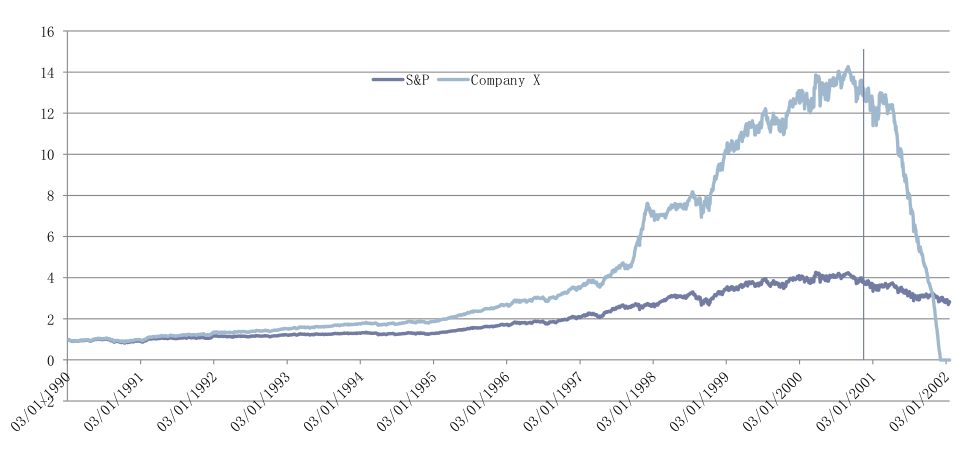
\includegraphics[scale=0.4]{../graph/exempleChuteEntreprise.png} \\
	    \caption{Exemple fictif d'une entreprise dont le cours augmente pendant de nombreuses années jusqu'au moment où le cours chute brutalement. La courbe bleue foncée représente un indice contenant l'entreprise X.}
	  \end{figure}
	  
L'exemple précédent mène à deux conclusions importantes : diversifier son portefeuille permet d'éviter les catastrophes et de réduire le risque sauf dans certains cas. En effet, en cas de crise économique, tous les actifs deviennent plus ou moins corrélés et chutent en même temps. Dans ce cas, on observerait probablement une chute générale des actifs du portefeuille comme on peut le voir sur le graphe suivant par exemple :
	  \begin{figure}[H]
	    \center
	    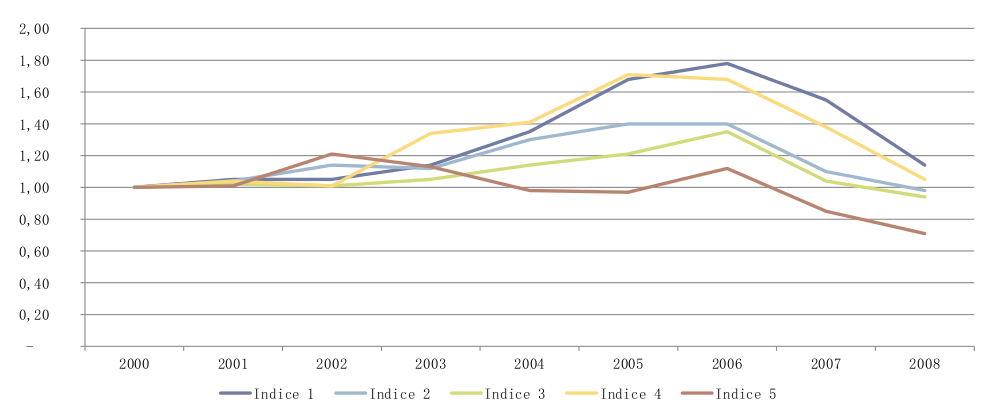
\includegraphics[scale=0.4]{../graph/exemplePortefeuilleChute.png} \\
	    \caption{Exemple fictif d'un portefeuille dont les actifs n'étaient au départ pas corrélés mais qui a la fin de 2006 ont tous chutés en même temps du fait de la crise.}
	  \end{figure}
Nous allons voir par la suite qu'un investissement est caractérisé par son rendement et sa volatilité (c'est-à-dire son rique).

\subsubsection{Les différents profils de risque}
Si l'on pose la question suivante à une population d'individus, on aura trois types de réponses :\\

\textit{Que choisissez-vous si l'on vous propose :
\begin{enumerate}
 \item Gagner 1 000\euro\ de manière certaine.
 \item Gagner 2 000\euro\ avec une chance sur deux.
\end{enumerate}
}
\noindent Dans les deux cas l'espérance de gain est de 1 000\euro\ . Voyons les différents types de réponse que l'ont peut avoir :
\begin{itemize}
 \item \underline{Les risk lovers/seekers :} ces personnes aiment le risque et auront tendance à choisir la deuxième possibilité.
 \item \underline{Les risk neutral :} ce sont les individus indécis. Souvent, ils regardent uniquement l'espérance de rendement et ne s'occupent pas vraiment du risque. Du coup, il ne savent pas choisir entre les deux propositions.
 \item \underline{Les risk adverse :} cette catégorie de personnes choisira la première solution sans hésiter puisque ce sont des individus averses au risque, il le fuit et veulent avoir un gain sûr minimal.
\end{itemize}
Bien sûr, nous nous sommes basé sur un exemple subjectif, le choix des personnes ne sera sans doute pas le même si l'on augmente le gain potentiel (100 000\euro\ ou 200 000\euro\ par exemple). En effet, on verra que beaucoup de personnes qui avaient choisi la deuxième possibilité ou étaient indécis vont alors choisir le premier choix. Cette notion dépend donc du capital de chaque individu. Néanmoins, cela donne une idée de la tolérance au risque de la personne. 

\subsubsection{La classification des actifs selon leur risque}
On distingue les actifs risqués des actifs moins risqués voir même des actifs dits 'sans risque'.
\begin{itemize}
 \item \textbf{Actifs 'sans risque' :} produits monétaires (prêts interbancaires, change à terme, swaps de taux d'intérêt, swaptions,...).
 \item \textbf{Actifs peu risqués :} ce sont les obligations, les emprunts d'Etats ou d'entreprise bien notée (de AAA à BBB).
 \item \textbf{Actifs risqués :} les obligations convertibles puis les actions.
 \item \textbf{Actifs très risqués :} les produits dérivés en général.
\end{itemize}
\begin{figure}[H]
  \center
  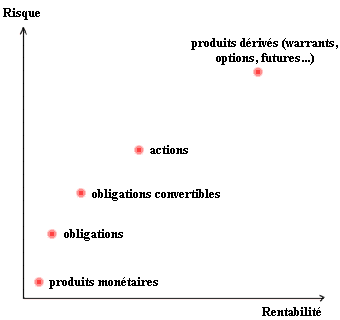
\includegraphics[scale=0.6]{../graph/actifsRisques.png}
  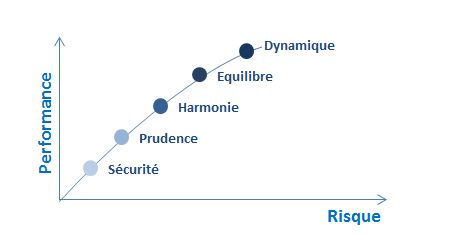
\includegraphics[scale=0.6]{../graph/profilsRisque.png}
  \caption{Graphe Risque/Rendement des différents types d'actifs - \url{http://www.abcbourse.com/apprendre/4_constituer_un_portefeuille2.html}}
\end{figure}


\subsection{L'évaluation d'un actif financier}
Un actif financier a la particularité de pouvoir être représenté par son rendement et son risque (ou volatilité). Nous allons donc voir comment les calculer.

\subsubsection{Le rendement}
Il existe deux types de rendements :
\begin{itemize}
 \item Les rendements périodiques/ponctuels : les dividendes, les coupons, les intérêts,...
 \item Les rendements continus : appréciation et dépréciation des actifs. On appelle cela le Profit \& Loss (P\&L), c'est le gain ou la perte en capital.
\end{itemize}

Il existe différentes manières de calculer le rendement d'un actif :
\begin{enumerate}
 \item \textbf{Le rendement Holding Period (sur la période de détention) :} c'est la différence entre le prix à la fin de la période et le prix au début, sommé avec les dividendes et le tout divisé sur le prix de départ.
 \[ R_{Holding Period} = \frac{Prix_{Fin}-Prix_{Debut}+dividendes}{Prix_{Debut}} \]
 En réalité cela donne un taux de rendement. Si on a invesit 1\euro\ au départ, on aura à la fin de la période \((1 + R_{Holding Period})\times 1\)\euro.
 \item \textbf{Le rendement arithmétique (ou moyen) :} c'est la moyenne des rendements $R_i$ sur plusieurs périodes.
 \[ R_{i} = \frac{1}{T} \sum_{t=1}^T R_{i,t}\]
 \item \textbf{Le rendement géométrique :} il est plus proche de la réalité que le rendement arithmétique qui lui fausse la vision que l'on a sur le vrai rendement.
 \[ R_{i} = \sqrt[T]{\prod_{k=1}^{T}(1+R_{i,k})}-1\]
 \item \textbf{Le Taux de Rendement Interne (TRI) :} c'est le taux d'actualisation qui annule la valeur actuelle nette (VAN) de la série des cash flows (flux de trésorerie).
 \[ VAN = \sum_{t=0}^{T} \frac{CashFlow}{(1+TRI)^t} = 0\]
 \item \textbf{Le rendement annualisé :} c'est le rendement d'une période ramené à un an.
 \[ R_{annuel} = (1+R_{periode})^C\]
 où $C$ est le nombre de périodes par an.
\end{enumerate}
Il existe d'autres types de rendements que nous ne détaillerons pas comme le rendement nominal avant ou après taxe.\\

Maintenant que l'on est capable de calculer le rendement d'un actif, on peut calculer le rendement d'un portefeuille composé de plusieurs actifs. Pour cela on définit les poids de chaque actifs $w_i$ et les rendements de chaques actifs $R_i$. Alors le rendement du portefeuille $R_P$ vaut :
\[ R_P = \sum_{i=1}^{N}w_iR_i\]
avec $N$ le nombre d'actifs différents du portefeuille et la somme des poids qui vaut 1 : \(\sum_{i=1}^{N}w_i =1\).

\subsubsection{La volatilité}


%Exemple bidon :
%Même rendement et volatilités différentes : on choisit la volatilité la plus faible si on est censé.
%Même volatilité et rendements différents : meilleur rendement.


%Analyse d'un historique : variance (volatilité)
%Covariance entre deux actifs
%Optimisation d'un portefeuille : Markowitz


%la VaR?

\subsection{La théorie moderne du portefeuille}
